\documentclass[10.5pt,a4paper]{article}
\usepackage[a4paper,margin=2cm]{geometry}
\usepackage{fontspec}
\usepackage{graphicx}
\usepackage{booktabs}
\usepackage{tabularx}
\usepackage{array}
\usepackage{multirow}
\usepackage{xcolor}
\usepackage{enumitem}
\usepackage[font=small,labelfont=bf]{caption}
\usepackage[numbers,sort&compress]{natbib}
\usepackage[hidelinks]{hyperref}
\usepackage{url}
\usepackage{pdflscape}
\usepackage[section]{placeins}
\usepackage{float}
\usepackage{afterpage}

\definecolor{qorange}{HTML}{C94401}
\newcommand{\file}[1]{\texttt{\small #1}}
\newcommand{\fn}[1]{\texttt{\small #1}}
\newcolumntype{L}[1]{>{\raggedright\arraybackslash}p{#1}}
\newcolumntype{Y}{>{\raggedright\arraybackslash}X}
\renewcommand{\arraystretch}{1.18}
\emergencystretch=3em
\newcommand{\openRate}{Mac 40,000 tasks/s, Server 9,000 tasks/s}
\newcommand{\throughputErrors}{Mac: 0, Server: 0}
\newcommand{\purgeMeasure}{Mac: \texttt{phys\_footprint}, Server: \texttt{rss}}
\newcommand{\ablationMacRuns}{5}
\newcommand{\capacityMacMeasure}{phys\_footprint}
\newcommand{\capacityServerMeasure}{rss}

\setlist{itemsep=2pt,topsep=4pt}
\makeatletter\newcommand{\rows}[1]{\@@input #1 }\makeatother

\title{\textbf{Quicx with an Adaptive Pool}\\[3pt]
\large Combining allocator research in a task queue that lives on a fixed memory budget}
\author{Dimitar Anastasov}
\date{November 2026 · branch \texttt{adaptive-pool}, apool v2}

\begin{document}
\maketitle

\begin{abstract}
\noindent
Quicx is a single-threaded task queue daemon written in C that never uses more memory than one budget fixed at start-up. Until version 1.0.4 that budget was split between block sizes by fixed percentages (PMAD), so most of it sat unused whenever the traffic did not match the split. This report describes \emph{apool v2}, an allocator whose 16~KiB pages move between block sizes as the traffic changes. It combines five ideas from the allocator literature, each behind a switch so it could be measured on its own, with two changes of my own. On an Apple M4 Pro with the default 8~MiB budget, the daemon holds 46,593 tasks of 100~B instead of 655, and 30,947 generated nginx log lines instead of 1,433. After a burst drains it keeps 2,080~KB of physical memory instead of 9,200~KB. Throughput and latency are unchanged within the run-to-run noise. The end-to-end tests also found a liveness bug in the released 1.0.4: once its queue is full of 16~B or 32~B tasks, a worker that connects afterwards can never register, so the queue can never be drained. One of the five ideas, fullest-page-first from Hoard, gave no benefit on queue traffic and is switched off. A second machine, a 2011 Intel Core i3 PC running Ubuntu Linux, reproduces every capacity number exactly, the 1.0.4 deadlock and the cost of purging (Section~\ref{sec:server}). All numbers come from raw logs in \file{results/}.
\end{abstract}

\section{Introduction}

A task queue sits between \emph{producers}, which submit work, and \emph{workers}, which do it. Quicx keeps every queued task in memory, and it promises never to grow beyond a configured budget: when the budget is full it refuses new work with \texttt{ERROR 0x01} instead of growing. That promise is only useful if the budget can actually be filled. A static split by block size cannot guarantee this. With the default PMAD configuration, a queue of 100~B tasks is refused after 655 tasks, while almost all of the 8~MiB is still free in other size classes.

The contribution of this work is engineering and measurement, not a new algorithm. Every mechanism used here exists in published allocators, and Section~\ref{sec:features} names the source of each. What is new for Quicx is:
\begin{itemize}
  \item an allocator that keeps the hard budget of the old design but lets pages move between sizes;
  \item five published ideas combined in it, each behind a flag, with a measured benefit and cost for each;
  \item a separate \emph{control pool} for connections and workers, which removes a liveness failure that the static design has;
  \item tests and benchmarks for every feature, run on real hardware, with the raw output kept.
\end{itemize}

\section{System overview}

Figure~\ref{fig:quicx} shows the whole daemon. One event loop (kqueue on macOS, epoll on Linux) wakes up when a socket is readable. \file{server.c} reads and checks each frame of QXP, the Quicx Protocol (a binary protocol designed for Quicx): a 6-byte header followed by a body of at most 1,024~B. \file{daemon.c} decides what each message means, and \file{dispacher.c} pairs waiting tasks with idle workers. The budget is split once at start-up by \fn{quicx\_init} (\file{quicx.c}): 3 pages (49,280~B) form the control pool for 1,024 connections and 1,024 workers, and the rest (8,339,328~B, 508 pages) is the task pool.

Both diagrams follow the C4 model's notation rules and review checklist \citep{brownc4}: a title that names the diagram type and scope, a legend for every colour, shape, border and line style, a type or technology for every element, and a label and one direction for every arrow.

A task is \emph{one block}: the 64~B \texttt{Task} record followed by the payload. \file{server.c} allocates the block before it reads the payload, so the payload is read straight into its final place. The dispatcher frees the block as soon as the \texttt{TASK} message is sent, which makes delivery at-most-once.

\afterpage{\begin{landscape}
\begin{figure}[p]
  \centering
  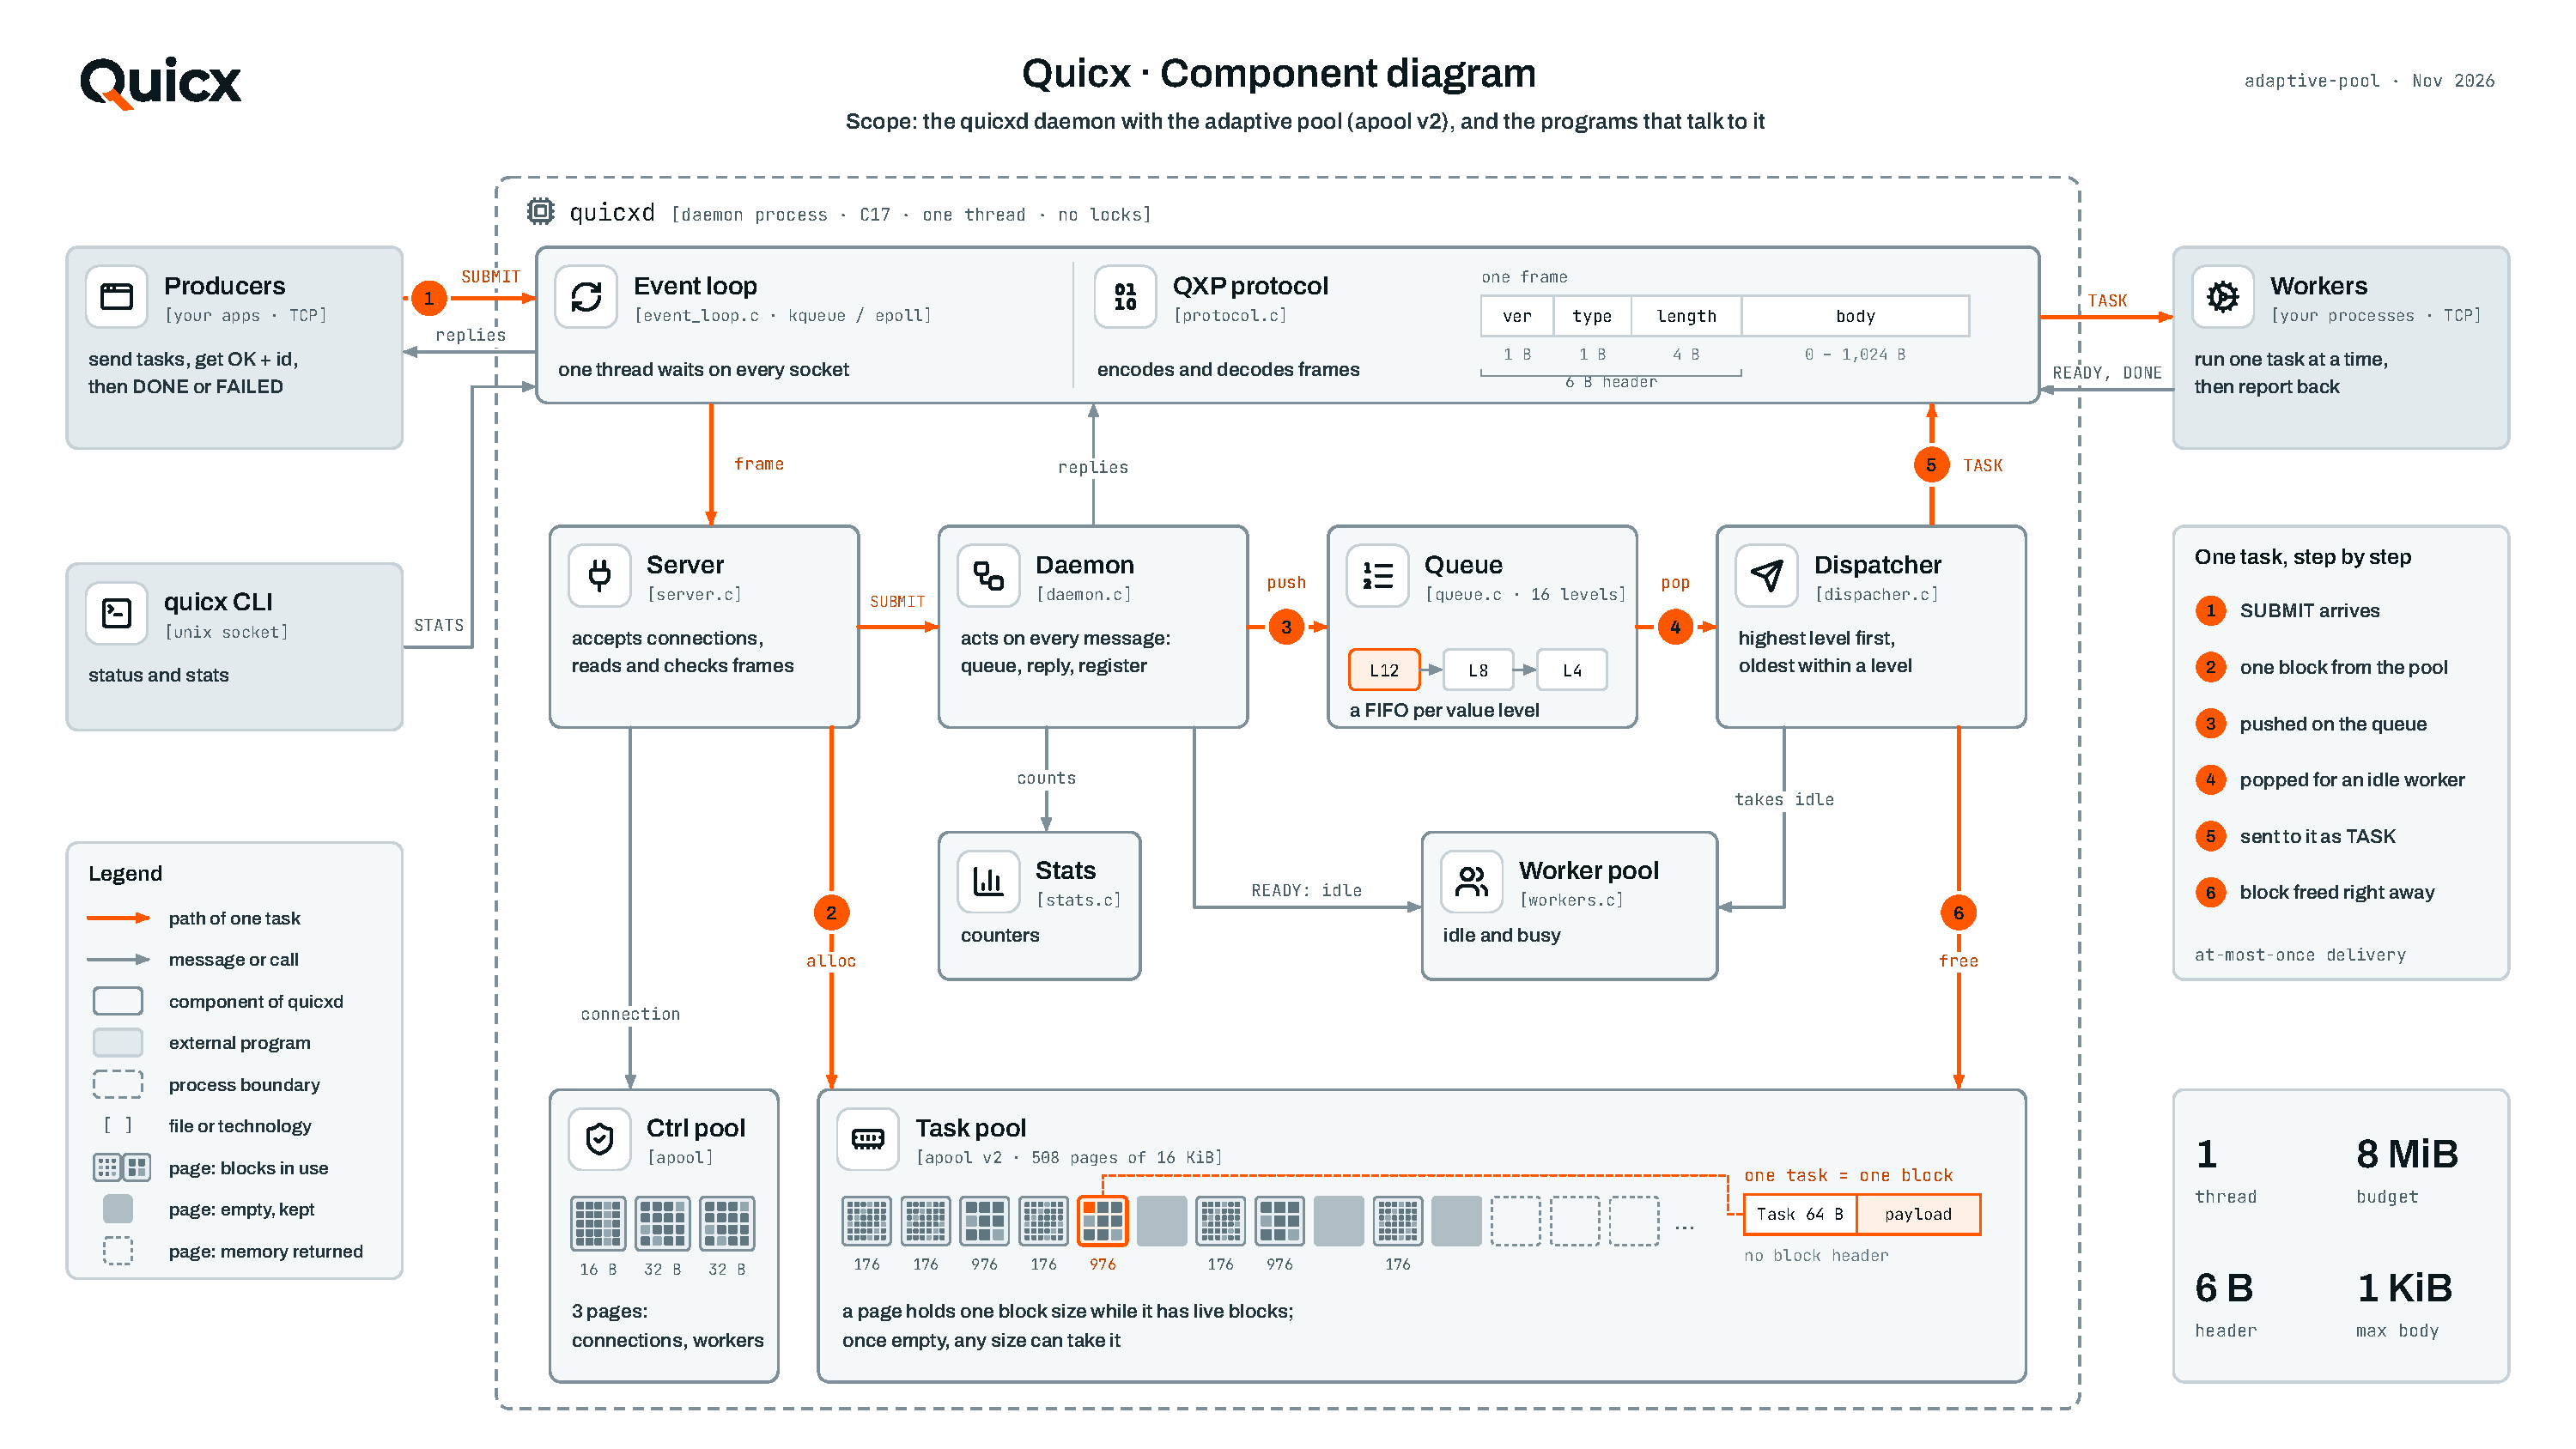
\includegraphics[width=\linewidth]{figures/quicx-architecture-light.pdf}
  \caption{Component diagram of Quicx with apool v2. Every element has a name, a \texttt{[file or technology]} tag and a one-line description; every arrow points from the sender and is labelled; the legend explains every fill, border and line style. Orange marks the path of one task, steps 1--6. Icons: Lucide (ISC licence). A dark version for slides and the website is in \file{figures/}.}
  \label{fig:quicx}
\end{figure}
\end{landscape}}

\section{The allocator}

Figure~\ref{fig:apool} shows apool v2 (\file{quicx/src/apool.c}, 341 lines). A pool is one \fn{mmap} that is never grown or moved. It is cut into 16~KiB pages, followed by one 32~B record per page. A page that is in use belongs to one block size (68 sizes, 16 to 1,088~B in steps of 16) and one lifetime class. Blocks carry no header. The page of a block is found by dividing its offset by 16,384, and the page's record holds everything else. Inside a page, freed blocks form a list through their own first 8 bytes, and blocks that were never used are handed out from a bump offset. When the last block of a page is freed, the page leaves its size and goes back to a shared free list, where \emph{any} size can take it next. That is the reshaping.

\afterpage{\begin{landscape}
\begin{figure}[p]
  \centering
  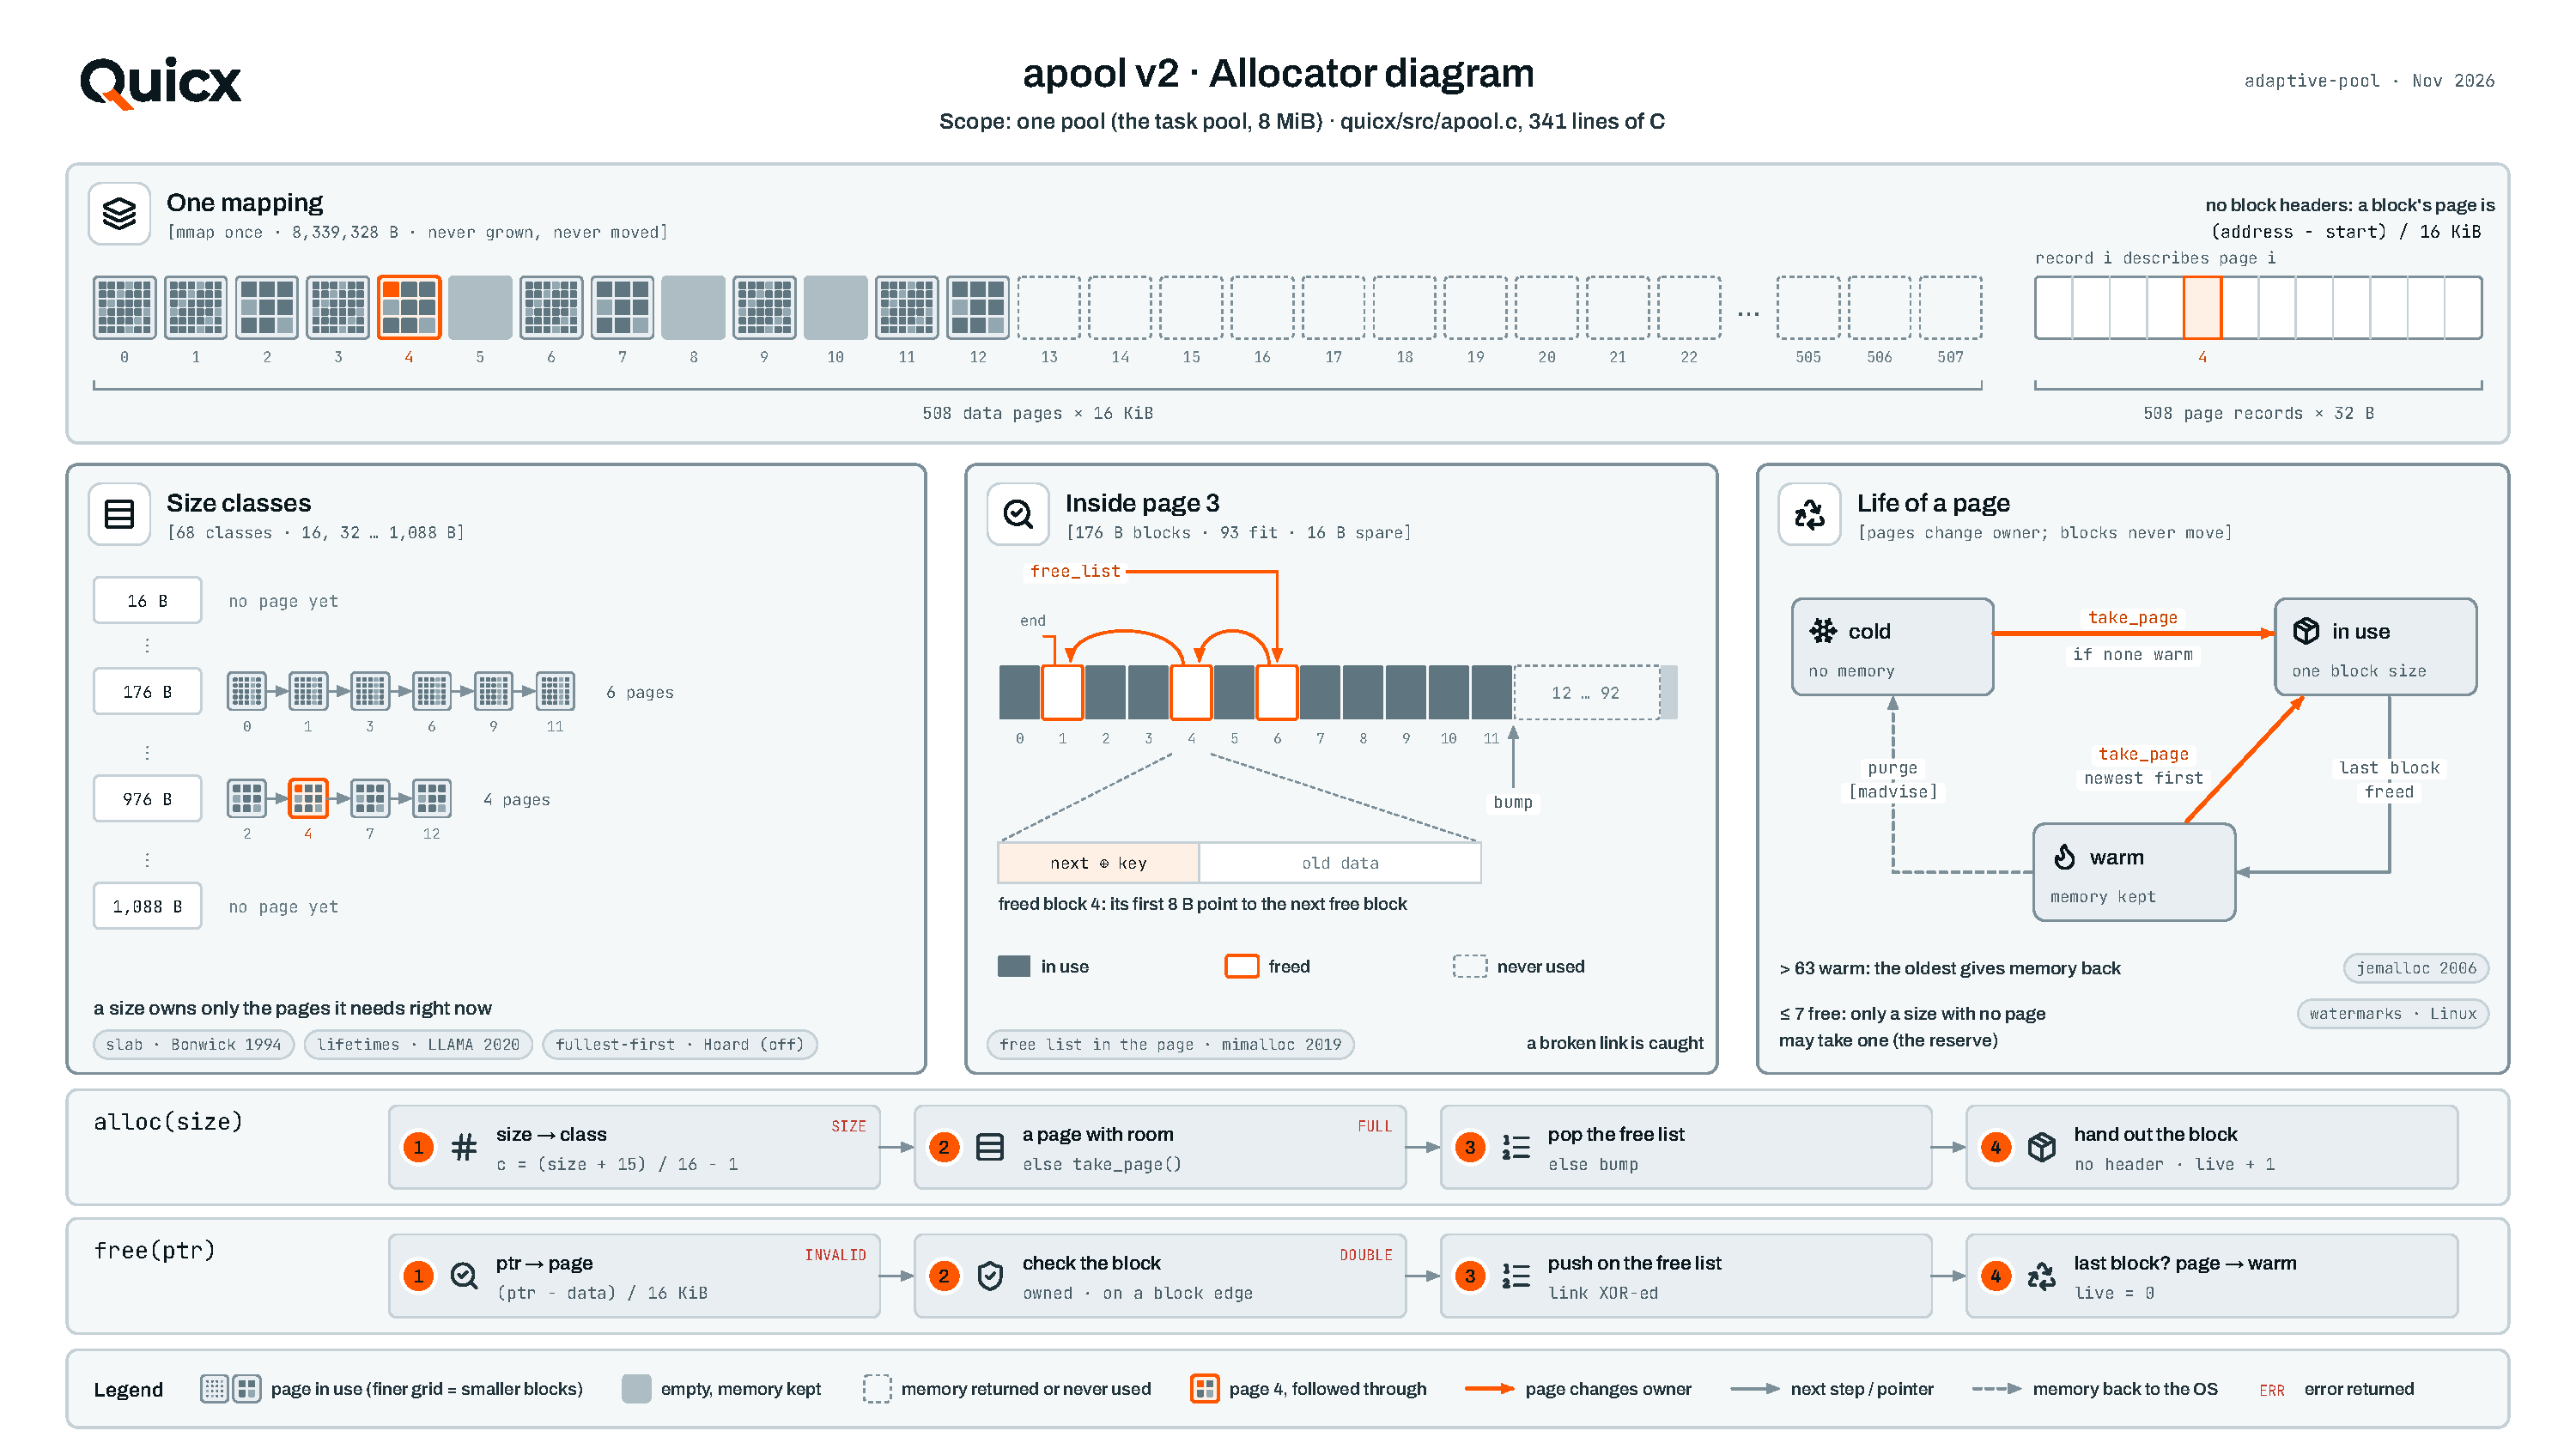
\includegraphics[width=\linewidth]{figures/apool-architecture-light.pdf}
  \caption{apool v2: the one mapping with its page records, the size classes and the pages each one owns, the inside of one page with its free list, the life of a page, and the alloc and free paths with the error each step can return. Page~4 is followed through every part. Grey tags name the paper each idea came from (Table~\ref{tab:features}).}
  \label{fig:apool}
\end{figure}
\end{landscape}}

\section{Features taken from papers}\label{sec:features}

Table~\ref{tab:features} lists every feature, where it came from, what it buys and where it is in the code. The flags are set per pool before the first allocation, and \texttt{APOOL\_F\_DEFAULT} is \texttt{RESERVE | HARDEN | PURGE}. Each feature can be switched in the \texttt{[allocator]} section of \file{quicx.conf} (\texttt{reserve}, \texttt{hardening}, \texttt{purge}, \texttt{fullest\_first}, plus \texttt{warm\_pages} and \texttt{reserve\_pages}); the file in the repository lists every key with its default, and \file{pool\_config.c} reads them into one \texttt{PoolConfig}.

\begin{table}[ht]
\centering
\footnotesize
\begin{tabularx}{\textwidth}{@{}L{2.25cm}L{2.3cm}YL{3.35cm}YL{1.15cm}@{}}
\toprule
Feature & Source & Benefit & Where (file, function) & How it works & Default \\
\midrule
Pages move between sizes (the core) & slab allocator \citep{bonwick1994slab}; mimalloc pages \citep{leijen2019mimalloc}; memcached \citep{memcached1411} & the same budget serves whatever sizes arrive & \file{apool.c}: \fn{take\_page} (l.~126), \fn{release\_page} (l.~157) & a size takes a free page only when it has no room; a page whose last block is freed returns to the shared list & always \\
Reserve & Linux zone watermarks \citep{gorman2004vmm}; memcached per-class minimum \citep{memcached1411} & one size cannot lock every other size out & \file{apool.c}: \fn{take\_page} (l.~128), \fn{apool\_init} (l.~208) & with $\le n/64$ free pages (7 of 508), only a size that owns no page may take one & on \\
Hardening & mimalloc secure mode \citep{leijen2019mimalloc} & corruption and double frees are detected, not silent & \file{apool.c}: \fn{encode}/\fn{decode} (l.~31), \fn{apool\_alloc\_hint} (l.~252), \fn{apool\_free} (l.~306) & free-list links are XOR-ed with a per-pool key; a decoded link must point into the same page; a block that looks freed triggers a bounded walk of its page's list & on \\
Purge with a warm list & jemalloc \citep{evans2006jemalloc}; mimalloc \citep{leijen2019mimalloc}; \texttt{madvise} \citep{linuxmadvise,xnumman} & memory goes back to the OS after a burst & \file{apool.c}: \fn{release\_page} (l.~165), \fn{purge}/\fn{unpurge} (l.~106) & empty pages are reused newest first; beyond $n/8$ empty pages (63 of 508) the coldest is purged (\texttt{MADV\_FREE\_REUSABLE} on macOS, \texttt{MADV\_DONTNEED} on Linux) & on \\
Lifetime classes & LLAMA \citep{maas2020llama} & a few long-lived blocks cannot pin pages full of short-lived ones & \file{apool.c}: \fn{apool\_alloc\_hint}, \fn{group\_head} (l.~59) & a caller marks a block as long-lived; such blocks get their own pages & available, unused \\
Fullest page first & Hoard \citep{berger2000hoard} & meant to let emptier pages drain so they can be reshaped & \file{apool.c}: \fn{group\_of}, \fn{regroup} (l.~64--76) & four fullness groups per size; allocation uses the fullest page & off \\
One block per task & own change & one allocation and one free per task; no record/payload split & \file{server.c}: \fn{handle\_readable} (l.~163); \file{dispacher.c} (l.~24) & the payload sits right behind the 64~B \texttt{Task} record & always \\
Control pool & own change; same principle as reserved memory for forward progress \citep{corbet2005ldd3} & a full task pool cannot stop workers from registering & \file{quicx.c}: \fn{quicx\_init} (l.~12--22); \file{server.c} l.~81; \file{daemon.c} l.~42 & Connections and Workers come from a separate 3-page pool sized for 1,024 of each & always \\
\bottomrule
\end{tabularx}
\caption{Features of apool v2, their sources, benefits and places in the code. Line numbers refer to the \texttt{adaptive-pool} worktree on 8 Nov 2026.}
\label{tab:features}
\end{table}

\paragraph{Pages move between sizes.} This is the slab idea \citep{bonwick1994slab}: memory is managed in pages, and each page holds blocks of one size. Like mimalloc's pages \citep{leijen2019mimalloc}, an empty page is not kept by its size but returned for any size to reuse. memcached reaches a similar effect by moving 1~MB pages between its classes in the background \citep{memcached1411}. apool only ever moves \emph{empty} pages, because a queue cannot evict a task the way a cache can evict an item.

\paragraph{Reserve.} Linux keeps a few pages per zone below a watermark for allocations that must succeed \citep{gorman2004vmm}. apool keeps the last $n/64$ free pages for sizes that own no page yet. Without it, a flood of one size takes every page and the next size is refused completely.

\paragraph{Hardening.} Following mimalloc's secure mode \citep{leijen2019mimalloc}, the address stored inside a free block is XOR-ed with a random per-pool key. A block overwritten after it was freed decodes to an address outside its page and is detected. A second free of the same block is found by walking that page's free list, which happens only when the block's first word looks like a link. The first word is cleared on every allocation, so a live block almost never looks like one.

\paragraph{Purge with a warm list.} jemalloc and mimalloc give unused memory back to the operating system \citep{evans2006jemalloc,leijen2019mimalloc}. Doing this on every empty page would put a system call on the hot path. apool keeps the $n/8$ most recently emptied pages \emph{warm} and purges only beyond that, oldest first.

\paragraph{Lifetime classes.} LLAMA predicts object lifetimes and groups objects by them \citep{maas2020llama}. apool takes the simple form of the idea: the caller passes a hint, and long-lived blocks get pages of their own. The daemon passes no hint today, because every task is freed in arrival order, so the feature is ready for redelivery, priorities or delayed tasks.

\paragraph{Fullest page first: a negative result.} Hoard sorts pages into fullness groups and allocates from the fuller ones so that the emptier ones drain \citep{berger2000hoard}. On queue traffic this did not help. Tasks are freed almost in arrival order, so pages already drain on their own, and the extra list moves cost time (Table~\ref{tab:ablation}). The feature stays in the code behind its flag and is off by default.

\section{Method}\label{sec:method}

\paragraph{Machines.} Table~\ref{tab:machines} lists the machines. Both machines ran the same scripts on 8 November 2026. Each built its own binaries with its own compiler. The Linux server is a much older and slower machine, which is useful: an effect that shows on both is not a property of one CPU or one kernel (Section~\ref{sec:server}).

\begin{table}[ht]
\centering\footnotesize
\begin{tabularx}{\textwidth}{@{}L{3cm}YY@{}}
\toprule
& Mac & Server \\
\midrule
\rows{tables/machines.tex}
\bottomrule
\end{tabularx}
\caption{Machines (from \file{results/*/machine.txt}).}
\label{tab:machines}
\end{table}

\paragraph{Versions.} \textbf{1.0.4} is the released version (tag \texttt{v1.0.4}, static PMAD pool \citep{pmad}). \textbf{v1} is the first adaptive pool from before the papers (commit \texttt{e7d4cdf}). \textbf{v2} is the current \texttt{adaptive-pool} worktree. All three daemons are built by \file{scripts/build.sh} with the same compiler and the release flags (\texttt{-std=c17 -O2}, as the CI release build uses). In the allocator-only benchmark, ``apool v1'' is the v2 code with every flag off and two blocks per task, which is how v1 behaved.

\paragraph{Repetitions.} The allocator benchmarks run 5 times, the page-size sweep 3 times and the end-to-end capacity runs 3 times. The throughput and latency runs are 5 runs per version, interleaved (1.0.4, v1, v2, 1.0.4, \dots) so that slow drift affects every version alike. Timings are reported as the median with the minimum and maximum in brackets. Counts that should not change between runs are printed once; a $\dagger$ would mark a count that changed, and none did.

\paragraph{Memory.} Physical memory is \texttt{phys\_footprint} on macOS (what \texttt{MADV\_FREE\_REUSABLE} lowers and what Activity Monitor shows), read with \texttt{vmmap} for the daemon and with \texttt{task\_info} inside \file{bench\_purge}. On Linux it is the resident set size from \file{/proc}.

\paragraph{Load.} The end-to-end clients are the C programs of the \texttt{bench} branch (commit \texttt{bfff3d0}, copied to \file{scripts/bench/}): 8 workers and 2 producer processes with 4 connections each, on the same machine as the daemon, over loopback. The payloads are nginx access-log lines generated by \file{workload.h}. Closed loop keeps 32 tasks in flight per connection. Open loop sends at a fixed rate (\openRate{}) and measures latency from the intended send time. Protocol errors and dropped connections reported by the producers, over all runs: \throughputErrors{}.

\section{Tests}\label{sec:tests}

Every feature has at least one test that shows it works. The tests are: \file{test\_apool} (50 checks, \file{quicx/src/tests/test\_apool.c}), \file{test\_wire} (28 checks), and the end-to-end checks in \file{scripts/e2e\_tests.py}, which drive a real daemon over TCP. Tables~\ref{tab:unit} and~\ref{tab:e2e} show the results.

\begin{table}[ht]
\centering\footnotesize
\begin{tabularx}{\textwidth}{@{}L{3.6cm}YL{2.6cm}L{1.4cm}L{1.4cm}@{}}
\toprule
Test & What it proves & Feature & Mac & Server \\
\midrule
\rows{tables/unit_tests.tex}
\bottomrule
\end{tabularx}
\caption{Unit tests of the allocator and the wire format (\file{results/*/test\_apool.txt}, \file{test\_wire.txt}).}
\label{tab:unit}
\end{table}

\begin{table}[ht]
\centering\footnotesize
\begin{tabularx}{\textwidth}{@{}L{1.9cm}YL{2.2cm}cccc@{}}
\toprule
& & & \multicolumn{2}{c}{Mac} & \multicolumn{2}{c}{Server} \\
\cmidrule(lr){4-5}\cmidrule(lr){6-7}
Test & What it checks & Feature & 1.0.4 & v2 & 1.0.4 & v2 \\
\midrule
\rows{tables/e2e_tests.tex}
\bottomrule
\end{tabularx}
\caption{End-to-end tests against real daemons (\file{results/*/e2e\_*.txt}). v1 passes the same checks as v2. Each test starts its own daemon.}
\label{tab:e2e}
\end{table}

\noindent The checks that failed, with the reason each test printed:
\begin{itemize}\small
\item Mac, 1.0.4, \texttt{liveness-16/late-worker-drains-all}: drained 0/5240; the daemon closed the worker's connection (no memory for it)
\item Mac, 1.0.4, \texttt{liveness-16/queue-usable-after}: type 3
\item Mac, 1.0.4, \texttt{liveness-32/late-worker-drains-all}: drained 0/3494; READY refused: 'worker pool full'
\item Mac, 1.0.4, \texttt{liveness-32/queue-usable-after}: type 3
\item Server, 1.0.4, \texttt{liveness-16/late-worker-drains-all}: drained 0/5240; the daemon closed the worker's connection (no memory for it)
\item Server, 1.0.4, \texttt{liveness-16/queue-usable-after}: type 3
\item Server, 1.0.4, \texttt{liveness-32/late-worker-drains-all}: drained 0/3494; READY refused: 'worker pool full'
\item Server, 1.0.4, \texttt{liveness-32/queue-usable-after}: type 3

\end{itemize}

\subsection{All features together}\label{sec:together}

Each feature is tested on its own above, but in the daemon they all run at the same time. Two checks show that they work together (Table~\ref{tab:together}). The allocator stress test makes 2 million random allocations and frees of 1 to 1,088~B, marks 1 in 8 blocks as long-lived and checks every byte of every block. It runs once with the daemon's features and once with every allocator feature on, fullest-first included. The daemon was also run with every feature on (\texttt{fullest\_first = on} in \file{quicx.conf}; the test build \texttt{quicxd-v2-all} makes that its default with \texttt{-DQUICX\_POOL\_FLAGS=APOOL\_F\_ALL}, \file{pool\_config.c}) and put through the same end-to-end tests and capacity runs. Nothing breaks and nothing changes: the counts are identical and memory still goes back after every burst.

In the daemon as shipped, six of the eight features run together all the time: pages moving between sizes, the reserve, hardening, purge, one block per task and the control pool. Fullest-first is off because it did not help (Section~\ref{sec:features}). Lifetime classes work in the allocator, but the daemon passes no hint yet.

\begin{table}[ht]
\centering\footnotesize
\begin{tabularx}{\textwidth}{@{}Yrrrr@{}}
\toprule
& \multicolumn{2}{c}{Mac} & \multicolumn{2}{c}{Server} \\
\cmidrule(lr){2-3}\cmidrule(lr){4-5}
& v2 & all features on & v2 & all features on \\
\midrule
\rows{tables/combined.tex}
\bottomrule
\end{tabularx}
\caption{The features working together: v2 as shipped against v2 with every allocator feature on (\file{results/*/test\_apool.txt}, \file{e2e\_v2-all.txt}, \file{capacity\_v2-all\_*.txt}).}
\label{tab:together}
\end{table}

\section{Benchmarks}\label{sec:bench}

Table~\ref{tab:catalogue} lists every benchmark, what it measures, which feature it tests and how to run it. The code is in the named files; it is not repeated in the tables.

\begin{table}[ht]
\centering\footnotesize
\begin{tabularx}{\textwidth}{@{}L{2.4cm}YL{3cm}L{3.2cm}@{}}
\toprule
Benchmark & What it measures & Feature / source & File, command \\
\midrule
capacity & 100~B tasks that fit in 8~MiB & core \citep{bonwick1994slab,leijen2019mimalloc} & \file{bench\_apool.c} \fn{w\_capacity}; \texttt{bench\_apool} \\
phases & tasks that fit as the size changes 100 $\to$ 900 $\to$ 40 $\to$ 300~B on one pool & core (reshaping) & \fn{w\_phases} \\
starve & 900~B tasks that still fit after 40~B tasks fill the pool & reserve \citep{gorman2004vmm} & \fn{w\_starve} \\
pinned & 900~B tasks that fit after 100~B tasks drain but 1 in 20 stays & lifetime classes \citep{maas2020llama} & \fn{w\_pin} \\
depth & deepest mixed-size queue (FIFO, 8 out of order, random) that never fails & fullest-first \citep{berger2000hoard}, fragmentation & \fn{w\_depth} \\
ns per task & alloc + free per task in a 1,000-deep FIFO churn & hardening \citep{leijen2019mimalloc}, one block per task & \fn{w\_speed} \\
page size & the above for 4--64~KiB pages & page size choice & \texttt{bench\_apool\_ps*} (\texttt{-DAPOOL\_PAGE\_SIZE}) \\
purge & physical memory full and after a drain; cost of pool-sized bursts; purges during steady churn & purge \citep{evans2006jemalloc,leijen2019mimalloc} & \file{bench\_purge.c}; \texttt{bench\_purge} \\
daemon capacity & tasks a real daemon accepts per phase (100, 900, 40, 300~B, nginx lines) and its physical memory & core, control pool, purge & \file{scripts/capacity.py} with the C client \file{fill.c} \\
throughput & closed-loop tasks/s, whole daemon & everything, end to end & \file{scripts/bench/run.sh -w 8 -p 2 -c 4 -i 32 -d 10 -u 2} \\
latency & p50 / p99 / p99.9 at a fixed rate & everything, end to end & \file{run.sh ... -r RATE} \\
\bottomrule
\end{tabularx}
\caption{Benchmark catalogue. \file{scripts/run\_all.sh MACHINE} runs all of them; \file{scripts/make\_tables.py} builds the tables below from the raw output.}
\label{tab:catalogue}
\end{table}

\section{Results}\label{sec:results}

\subsection{Allocator ablation}

Table~\ref{tab:ablation} compares PMAD, v1, v2 and v2 with one feature switched off (or on), in one 8~MiB pool, on the Mac (\ablationMacRuns{} runs).

\begin{table}[ht]
\centering\footnotesize
\setlength{\tabcolsep}{4pt}
\begin{tabularx}{\textwidth}{@{}Yrrrrrrrrr@{}}
\toprule
& \multicolumn{4}{c}{tasks that fit (capacity, then phases)} & & & \multicolumn{2}{c}{deepest queue} & \\
\cmidrule(lr){2-5}\cmidrule(lr){8-9}
Allocator & 100~B & 900~B & 40~B & 300~B & starve & pinned & FIFO & random & ns/task \\
\midrule
\rows{tables/ablation_mac.tex}
\bottomrule
\end{tabularx}
\caption{Allocator-only ablation on the Mac (\file{results/mac/bench\_apool\_*.txt}). ns/task: median and range of the runs; the other columns were identical in every run.}
\label{tab:ablation}
\end{table}

\noindent What each line shows:
\begin{itemize}
  \item \textbf{Core.} v2 holds 46,872 tasks of 100~B where PMAD holds 655, about 71 times more, and it follows every change of size.
  \item \textbf{Reserve.} Without it, a size arriving after a flood gets nothing (0). With it, the new size gets one page (16 tasks of 900~B). This costs 651 tasks of capacity at 100~B (47,523 $\to$ 46,872, 1.4\%).
  \item \textbf{Lifetime hints.} With hints, 7,648 tasks of 900~B fit after the pinning pattern; without them, 16.
  \item \textbf{Hardening} costs about 1~ns per task (13.8 $\to$ 14.8).
  \item \textbf{One block per task} saves about 10~ns per task (24.5 $\to$ 14.8).
  \item \textbf{Fullest-first} lowers the deepest FIFO queue (29,952 $\to$ 29,696) and costs about 5~ns per task.
\end{itemize}
The server's version of this table is in Appendix~\ref{app:server}.

\subsection{Purge}

\begin{table}[ht]
\centering\footnotesize
\begin{tabularx}{\textwidth}{@{}L{1.3cm}Yrrrrr@{}}
\toprule
& & full (KB) & after drain (KB) & burst ns/block & churn ns/task & churn purges \\
\midrule
\rows{tables/purge.tex}
\bottomrule
\end{tabularx}
\caption{\file{bench\_purge}: physical memory of the process above its baseline, with the pool full of 964~B blocks and after all are freed; time per block over 40 pool-sized bursts; time per task in steady churn (1,000 in flight). Memory measure: \purgeMeasure{}.}
\label{tab:purge}
\end{table}

Purging works as intended. After a drain the pool holds 1,104~KB above baseline instead of 8,096~KB, and steady churn never purges (0 purges, same time per task). The cost is on bursts that fill and empty the \emph{whole} pool again and again. Each such burst purges 441 pages and brings them back, which costs 102~ns per block instead of 8.7 (Section~\ref{sec:findings}). The server shows the same trade-off at its own speed: 584.7 instead of 51.1~ns per block, again about 11 times more, and 1,280~KB instead of 8,080~KB after a drain.

\subsection{Page size}

\begin{table}[ht]
\centering\footnotesize
\begin{tabularx}{\textwidth}{@{}Yrrrrrrrr@{}}
\toprule
& \multicolumn{4}{c}{Mac} & \multicolumn{4}{c}{Server} \\
\cmidrule(lr){2-5}\cmidrule(lr){6-9}
Page & 100~B & starve & FIFO depth & ns/task & 100~B & starve & FIFO depth & ns/task \\
\midrule
\rows{tables/pagesize.tex}
\bottomrule
\end{tabularx}
\caption{apool v2 with other page sizes (\file{results/*/bench\_ps*\_*.txt}).}
\label{tab:pagesize}
\end{table}

Smaller pages make every page change cost relatively more (22.2~ns per task at 4~KiB) and give a new size fewer blocks from the reserve. Larger pages waste more space at the end of each size's last page, so the deepest mixed queue falls from 29,952 (16~KiB) to 23,680 (64~KiB). 16~KiB is the best balance of the sizes tried, and it is also the OS page size on Apple Silicon, so one apool page is exactly one OS page to purge. The server gives the same counts and the same order of times (78.3~ns per task at 4~KiB, 72.9 at 16~KiB, no gain beyond).

\subsection{Whole daemon: capacity and memory}

\begin{table}[ht]
\centering\footnotesize
\setlength{\tabcolsep}{4pt}
\begin{tabularx}{\textwidth}{@{}Yrrrrrrrrc@{}}
\toprule
& \multicolumn{5}{c}{tasks accepted before ERROR 0x01} & \multicolumn{3}{c}{physical memory (KB)} & \\
\cmidrule(lr){2-6}\cmidrule(lr){7-9}
Version & 100~B & 900~B & 40~B & 300~B & nginx & idle & full & after drain & all drained \\
\midrule
\rows{tables/capacity_mac.tex}
\bottomrule
\end{tabularx}
\caption{One daemon per version, phases in this order, 8~MiB budget, Mac (\file{results/mac/capacity\_*.txt}, 3 runs). ``after drain'' is after the last phase. Memory measure: \texttt{\capacityMacMeasure{}}.}
\label{tab:capacity}
\end{table}

The daemon numbers match the allocator benchmark, minus the 3 pages that now belong to the control pool. 1.0.4 holds its full 9,200~KB from the moment it starts, because PMAD writes a header into every block at start-up. v1 starts small but keeps whatever a burst touched. v2 starts at 1,056~KB and returns to 2,080~KB after every burst. The server repeats the pattern in resident memory (Appendix~\ref{app:server}): 1.0.4 holds 9,928~KB throughout, v1 grows from 1,784 to 9,916~KB and stays there, and v2 grows to 9,816~KB during the burst and returns to 2,736~KB.

\subsection{Throughput and latency}

\begin{table}[ht]
\centering\footnotesize
\begin{tabularx}{\textwidth}{@{}L{1.3cm}Yrrrr@{}}
\toprule
& & closed loop & \multicolumn{3}{c}{open loop at a fixed rate} \\
\cmidrule(lr){3-3}\cmidrule(lr){4-6}
Machine & Version & tasks/s & p50 µs & p99 µs & p99.9 µs \\
\midrule
\rows{tables/throughput.tex}
\bottomrule
\end{tabularx}
\caption{Closed-loop throughput and open-loop latency (rate: \openRate{}), median and range of 5 interleaved runs per version (\file{results/*/closed\_*.txt}, \file{open\_*.txt}).}
\label{tab:throughput}
\end{table}

The three versions are within each other's run-to-run range on every column. A task's round trip through the daemon takes about 12~µs, and the allocator's share of that, about 15~ns, is below the noise. On the server all three versions reach 19.0k tasks/s. There, eleven processes (the daemon, 8 workers and 2 producers) share 4 hardware threads, so the CPU is the limit and the three versions cannot be told apart. The new allocator did not make Quicx faster or slower on either machine; it changed how much fits and how much memory stays in use.

\section{Server runs}\label{sec:server}

The second machine is \texttt{da}, a desktop PC from 2011 (Intel Core i3-2100, 2 cores and 4 threads, 7.6~GiB, Ubuntu 24.04, gcc 13.3), reached over Tailscale. \file{scripts/run\_server.sh} copied the source to \file{\textasciitilde/quicx-report/} on it, built everything there with its own compiler, ran the same suite unattended (about 14 minutes) and copied \file{results/server/} back. Its results stand next to the Mac's in every table above and in Appendix~\ref{app:server}. What the second machine adds:
\begin{itemize}
  \item \textbf{Capacity is a property of the allocator, not of the machine.} Every count of tasks that fit is the same on both machines, in the allocator benchmark and in the whole daemon, even though the OS page size differs (16~KiB and 4~KiB).
  \item \textbf{The 1.0.4 deadlock is not specific to macOS.} \texttt{liveness-16} and \texttt{liveness-32} fail on Linux with the same messages (0 of 5,240 and 0 of 3,494 tasks drained).
  \item \textbf{Memory follows the same pattern} in resident set size: only v2 gives its memory back after a burst (2,736~KB, against 9,916~KB for v1 and 9,928~KB for 1.0.4).
  \item \textbf{Purge and hardening cost more on the older CPU} (584.7 against 51.1~ns per block in full-pool bursts; 13~ns per task for hardening). On Linux, \texttt{MADV\_DONTNEED} drops the pages, so each one is faulted in and zeroed again on reuse.
  \item \textbf{Throughput and latency do not separate the versions} here either: 19.0k tasks/s each, limited by 4 hardware threads.
\end{itemize}

\section{Findings}\label{sec:findings}

\begin{enumerate}
  \item \textbf{The released 1.0.4 can deadlock.} With PMAD, a 16~B payload shares a size class with \texttt{Connection} (16~B), and a 32~B payload with \texttt{Worker} (32~B). If the queue fills with such tasks before a worker is connected, the next worker is either disconnected at once (no memory for its \texttt{Connection}) or refused at READY (``worker pool full''). The queue can then never be drained until the daemon restarts (Table~\ref{tab:e2e}). v1 and v2 pass these tests because of the control pool. A 1.0.5 should either take the same fix or reserve PMAD blocks for connections and workers.
  \item \textbf{Purge has a burst cost.} When the whole pool is filled and emptied repeatedly, every cycle purges and re-uses 441 pages (about 1~µs each), so a burst costs 102 instead of 8.7~ns per block on the Mac, and 584.7 instead of 51.1~ns on the server. For the daemon, one such full cycle of 8,064 tasks takes far longer than the extra 0.8~ms, so the effect is small, but a workload of exactly this shape would pay for it. Raising \texttt{warm} or purging only after a delay, as jemalloc does, would reduce it.
  \item \textbf{Hardening costs more on an older CPU.} On the M4 Pro the encoded links and checks cost about 1~ns per task (13.8 $\to$ 14.8). On the i3-2100 they cost about 13~ns (60.0 $\to$ 72.8, 21\%) (Appendix~\ref{app:server}). The daemon's throughput is the same either way, because the allocator is a tiny part of a round trip. PMAD's fixed lists stay the fastest per allocation on both machines (13.3~ns and 43.3~ns); apool pays for its capacity with these extra nanoseconds.
  \item \textbf{Fullest-first does not help queue traffic} (Section~\ref{sec:features}) and is off.
  \item \textbf{Lifetime classes are unused by the daemon.} They fix the pinned case only when a caller passes a hint, and today every task is freed in arrival order.
  \item \textbf{The reserve costs capacity}: 1.4\% at 100~B, and 2.5\% of the deepest mixed queue.
  \item \textbf{Open-loop tail latency varies between runs on both machines.} For the \emph{same} version, p99.9 ranged from 129 to 4,470~µs on the Mac and from 137 to 4,296~µs on the server. The medians of the five runs are close (143--252~µs on the Mac, 207--214~µs on the server), and no version is consistently worse.
  \item \textbf{The branch reported version 1.0.3} while these runs were made, because it was made before the 1.0.4 version bump. It is 2.0.0 now (\file{quicx/include/cli.h}).
\end{enumerate}

\section{Threats to validity}

\begin{itemize}
  \item \textbf{Synthetic load.} The workloads are synthetic: fixed sizes, a random size mix, and nginx lines generated by a program rather than taken from a real log. Real traffic may mix sizes differently.
  \item \textbf{Two machines.} One Mac and one Linux PC. Other CPUs and kernels may differ. On the server the CPU frequency governor (\texttt{schedutil}) could not be fixed without root access, so its timings include frequency changes.
  \item \textbf{Shared CPU.} Clients and daemon share one machine over loopback, so they compete for CPU. Absolute throughput is a property of this setup, not of Quicx alone, which is why only the differences between versions are interpreted.
  \item \textbf{Different memory measures.} \texttt{phys\_footprint} (macOS) and resident set size (Linux) are not the same measure, so memory numbers should be compared within one machine only.
  \item \textbf{v1 is emulated in the allocator benchmark.} In \file{bench\_apool}, ``v1'' is v2's code with its features off. The end-to-end v1 is the real commit.
  \item \textbf{One thread.} The daemon is single-threaded. None of the published allocators' multi-thread features were needed or tested.
\end{itemize}

\section{Conclusion}

Combining published allocator ideas inside a fixed budget made the budget usable. The same 8~MiB holds about 71 times more 100-byte tasks, it follows changes in task size without a restart, and its memory goes back to the operating system after a burst, all without changing throughput or latency, on a 2024 Mac and on a 2011 Linux PC alike. Measuring each idea on its own showed which ones matter for a queue. The reserve and lifetime classes fix specific failure patterns, hardening is cheap safety, purge has a small cost on full-pool bursts, and fullest-first is not worth it. The tests also showed that the released 1.0.4 can deadlock with small tasks, which the control pool fixes.

\bibliographystyle{plainnat}
\bibliography{refs}

\appendix
\section{Server tables}\label{app:server}

\begin{table}[H]
\centering\footnotesize
\setlength{\tabcolsep}{4pt}
\begin{tabularx}{\textwidth}{@{}Yrrrrrrrrr@{}}
\toprule
Allocator & 100~B & 900~B & 40~B & 300~B & starve & pinned & FIFO & random & ns/task \\
\midrule
\rows{tables/ablation_server.tex}
\bottomrule
\end{tabularx}
\caption{Allocator-only ablation on the server (\file{results/server/bench\_apool\_*.txt}).}
\end{table}

\begin{table}[H]
\centering\footnotesize
\setlength{\tabcolsep}{4pt}
\begin{tabularx}{\textwidth}{@{}Yrrrrrrrrc@{}}
\toprule
Version & 100~B & 900~B & 40~B & 300~B & nginx & idle & full & after drain & all drained \\
\midrule
\rows{tables/capacity_server.tex}
\bottomrule
\end{tabularx}
\caption{Whole-daemon capacity and memory on the server. Memory measure: \texttt{\capacityServerMeasure{}}.}
\end{table}

\section{Reproducing}

\begin{verbatim}
cd docs/report
scripts/build.sh mac            # binaries into build/mac/
scripts/run_all.sh mac          # raw output into results/mac/ (about 10 minutes)
scripts/run_server.sh           # the same on the server, results copied back
python3 scripts/make_tables.py  # tables/ from results/
scripts/export_figures.sh       # diagrams: SVG, PDF, PNG, outlined SVG
tectonic -X compile main.tex    # this PDF
\end{verbatim}

\end{document}
